\documentclass[
oneside,titlepage,numbers=noenddot,headinclude,%1headlines,
footinclude=true,cleardoublepage=empty,
BCOR=5mm,paper=a4,fontsize=11pt, % Binding correction, paper type and font size
american % Languages, change this to your language(s)
]{scrartcl} 
\usepackage[american]{babel}      
\usepackage{graphicx}                 
\usepackage{amssymb,amsmath,amsfonts}
\usepackage{vmargin}
\usepackage{lmodern}
\usepackage{setspace}
\usepackage{multirow}
\usepackage{upgreek}
\usepackage{mathtools}
\usepackage[T1]{fontenc}
\usepackage{siunitx}
\usepackage{multirow}
%\usepackage{subcaption}
\usepackage{hyperref}
\usepackage{bm}
\usepackage[capbesideposition={inside,center},facing=yes,capbesidesep=quad]{floatrow}
%\usepackage{sidecap}
\usepackage[backend=biber, bibencoding=utf8,style=alphabetic, maxalphanames=1, minalphanames=1, maxnames=99, doi=false, isbn=false, url=false, backref=true]{biblatex}
\setkomafont{captionlabel}{%
	\textsc}%
\setcapindent{0em}

\addbibresource{PCA_report.bib}
% modified version of thomas uehlinger's phys-thomas.bbx file
% Sebi, 2015-10-26

% to get rid of the "+" after the first three letters, indicating that there were more than one author
\renewcommand*{\labelalphaothers}{}
\renewcommand\labelnamepunct{\addcomma\space}

% to have commas instead of semicolon between biblabels in multicite
\renewcommand\multicitedelim{\addcomma\space}

% to have only first three letters of first author
\DeclareLabelalphaTemplate{
  \labelelement{
    \field[final]{shorthand}
    \field{label}
    \field[strwidth=3,strside=left]{labelname}
  }
  \labelelement{
    \field[strwidth=2,strside=right]{year}    
  }
}


% suppress note
\AtEveryBibitem{%
  \clearfield{note}%
}

% suppress all DOI because there are a few left although they should be deactivated above
\AtEveryBibitem{%
  \clearfield{doi}%
}

% from Thomas:

% New options
\newtoggle{bbx:articletitle}
\newtoggle{bbx:chaptertitle}
\newtoggle{bbx:pageranges}
\DeclareBibliographyOption{articletitle}[true]{%
  \settoggle{bbx:articletitle}{#1}%
}
\DeclareBibliographyOption{chaptertitle}[true]{%
  \settoggle{bbx:chaptertitle}{#1}%
}
\DeclareBibliographyOption{pageranges}[true]{%
  \settoggle{bbx:pageranges}{#1}%
}
\DeclareBibliographyOption{biblabel}{%
  \ifstrequal{#1}{brackets}
    {%
      \DeclareFieldFormat{labelnumberwidth}{\mkbibbrackets{##1}}%
      \setlength{\biblabelsep}{10 pt}%
    }
    {%
      \DeclareFieldFormat{labelnumberwidth}{\mkbibsuperscript{##1}}%
      \setlength{\biblabelsep}{0 pt}%
    }%
}


% Alter settings that carry through from biblatex
\ExecuteBibliographyOptions
  {
    articletitle = true       ,
    chaptertitle = true       ,
    biblabel     = superscript,
    doi          = false      ,
    eprint       = false      ,
    giveninits   = true       ,
    isbn         = false      ,
    maxnames     = 999        ,
    maxcitenames = 2          ,
    url          = false      
  }


\renewbibmacro*{name:first-last}[4]{%
  \usebibmacro{name:delim}{#2#3#1}%
  \usebibmacro{name:hook}{#2#3#1}%
  \ifblank{#2}{}{\mkbibnamefirst{#2}\isdot\bibnamedelimd}%
  \ifblank{#3}{}{%
    \mkbibnameprefix{#3}\isdot
    \ifpunctmark{'}
      {}
      {\ifuseprefix{\bibnamedelimc}{\bibnamedelimd}}}%
  \mkbibnamelast{#1}\isdot
  \ifblank{#4}{}
    {\addcomma\space\mkbibnameaffix{#4}\isdot}%
}


		 		 
% Custom field formats
\DeclareFieldFormat[inproceedings]{booktitle}{#1}
\DeclareFieldFormat{eprint:arxiv}{%
  \ifhyperref
    {\href{http://arxiv.org/\abx@arxivpath/#1}{%
        \texttt{arXiv\addcolon}
        \nolinkurl{#1}%
        \iffieldundef{eprintclass}
	 {}
	 {\addspace\UrlFont{\mkbibbrackets{\thefield{eprintclass}}}}}}
    {\texttt{arXiv\addcolon}
      \nolinkurl{#1}
      \iffieldundef{eprintclass}
        {}
        {\addspace\UrlFont{\mkbibbrackets{\thefield{eprintclass}}}}}}
\DeclareFieldAlias{eprint:arXiv}{eprint:arxiv}
\DeclareFieldFormat[online]{date}{\mkbibparens{#1}\nopunct}
\DeclareFieldFormat{doi}{%
  \ifhyperref
    {\href{http://dx.doi.org/#1}{\nolinkurl{DOI:#1}}}
    {\nolinkurl{DOI:#1}}%
}
% \DeclareFieldFormat{doi/url-link}{% % uncomment this paragraph because it makes "firstofone" appear in the disorder2015 paper, dont know why
%   \ifhyperref
%     {%
%       \iffieldundef{doi}
%         {%
%           \iffieldundef{url}
%             {\@firstofone}
%             {\href{\thefield{url}}}%
%         }
%         {%
% 			\iftoggle{bbx:doi}%
% 				{\@firstofone}%
% 				{\href{http://dx.doi.org/\thefield{doi}}}%
% 		}%
%     }
%     {\@firstofone}%
%       {#1}%
% }
\DeclareFieldFormat{journaltitle}{#1\isdot}
\DeclareFieldFormat[article]{pages}{%
  \iftoggle{bbx:pageranges}{#1}{\mkfirstpage{#1}}%
}
\DeclareFieldFormat[article,inproceedings,patent,online,thesis,unpublished]{title}{%
  \iftoggle{bbx:articletitle}
    {\mkbibemph{#1\isdot}}
    {}%
}
\DeclareFieldFormat[incollection]{title}{%
  \iftoggle{bbx:chaptertitle}
    {\mkbibemph{#1\isdot}}
    {}%
}
\DeclareFieldFormat{related:translatedas}{\mkbibbrackets{#1}}
% \DeclareFieldFormat{titlecase}{\MakeSentenceCase{#1}} % had to uncomment here so that e.g. "Physical Review A" appears insteaf of "Physical review a"
\DeclareFieldFormat{url}{\url{#1}}
\DeclareFieldFormat[article]{volume}{\mkbibbold{#1}}
\DeclareFieldFormat{year}{\mkbibparens{#1}}
\DeclareFieldFormat{rawyear}{#1}

% macro to show the year including an a,b,c,... added to distinguish the labels in authoryear style
\newbibmacro{year+extrayear}{%
    \iffieldundef{\thefield{datelabelsource}year}
      {}
      {\printtext[parens]{%
         \printfield[rawyear]{year}%
         \printfield{extrayear}}}}%
		 
% Simple modifications to punctuation, etc.
\renewcommand*{\intitlepunct}{\addspace}
\providecommand*{\mkibid}[1]{#1}
\renewcommand*{\newunitpunct}{\addcomma\space}

% Bibliography strings
\DefineBibliographyStrings{english}{%
  andothers   = \mkbibemph{et al\adddot},
  byeditor  = edited by,
  chapter   = Chap\adddot,
  volume    = Vol\adddot
}

% Bibliography macros
\renewbibmacro*{chapter+pages}{%
  \setunit{\addspace}%
  \printfield{chapter}%
  \setunit{\bibpagespunct}%
  \printfield{pages}%
  \newunit
}

\renewbibmacro*{institution+location+date}{%
  \setunit{\addspace}%
  \printtext[parens]{%
    \printlist{institution}%
    \newunit
    \printlist{location}%
    \newunit
    \usebibmacro{date}%
	\printfield{extrayear}%
  }%
}

\renewbibmacro*{journal+issuetitle}{%
  \usebibmacro{journal}%
  \setunit*{\addspace}%
  \iffieldundef{series}
    {}
    {\newunit
     \printfield{series}%
     \setunit{\addspace}}%
  \usebibmacro{volume+number+eid}%
  \setunit{\addspace}%
  \usebibmacro{issue}%
  \newunit
}

\renewbibmacro*{maintitle+booktitle}{%
  \printtext[doi/url-link]{%
    \iffieldundef{maintitle}
      {}
      {%
        \usebibmacro{maintitle}%
        \newunit
      }%
    \usebibmacro{booktitle}%
  }%
  \newunit\newblock
  \iffieldundef{volume}
    {}
    {%
      \printfield{volume}%
      \clearfield{volume}%
      \printfield{part}%
      \clearfield{part}%
    }%
  \newunit
}

\newbibmacro*{organization+date}{%
  \setunit{\addspace}%
  \printtext[parens]{%
    \printlist{organization}%
    \newunit
    \usebibmacro{date}%
	\printfield{extrayear}%
  }%
  \newunit
}

\renewbibmacro*{publisher+location+date}{%
  \setunit{\addspace}%
  \printtext[parens]{%
    \printlist{publisher}%
    \newunit
    \printlist{location}%
    \newunit
    \usebibmacro{date}%
	\printfield{extrayear}%
  }%
  \newunit
}

\renewbibmacro*{volume+number+eid}{%
  \printfield{volume}%
  \newunit
  \printfield{eid}%
}

% New bibliography drivers, using the required order of fields. These
% are mainly copied from standard.bbx then modified.
\DeclareBibliographyDriver{article}{%
  \usebibmacro{bibindex}%
  \usebibmacro{begentry}%
  \usebibmacro{author/translator+others}%
  \setunit{\labelnamepunct}\newblock
  \usebibmacro{title}%
  \newunit\newblock
  \usebibmacro{byauthor}%
  \newunit\newblock
  \usebibmacro{bytranslator+others}%
  \newunit\newblock
  \printfield{version}%
  \newunit\newblock
  \printtext[doi/url-link]{%
    \usebibmacro{journal+issuetitle}%
    \newunit
    \usebibmacro{byeditor+others}%
    \newunit
    \usebibmacro{note+pages}%
    \newunit\newblock
    \iftoggle{bbx:isbn}
      {\printfield{issn}}
      {}%
    \setunit{\addspace}%
	\usebibmacro{year+extrayear}%
    %\printfield{year}%
	%\printfield{extrayear}%
  }%
  \setunit{\addspace}%
  \iffieldundef{pages}
    {%
      \printfield{doi}%
      \clearfield{doi}%
    }%
    {}%
  \newunit\newblock%
  \usebibmacro{doi+eprint+url}%
  \newunit\newblock
  \usebibmacro{addendum+pubstate}%
  \setunit{\bibpagerefpunct}\newblock
  \usebibmacro{pageref}%
  \newunit\newblock
  \usebibmacro{related}%
  \usebibmacro{finentry}%
}

\DeclareBibliographyDriver{unpublished}{%
  \usebibmacro{bibindex}%
  \usebibmacro{begentry}%
  \usebibmacro{author}%
  \setunit{\labelnamepunct}\newblock
  \usebibmacro{title}%
  \newunit
  \printlist{language}%
  \newunit\newblock
  \usebibmacro{byauthor}%
  \newunit\newblock
  \printfield{howpublished}%
  \newunit\newblock
  \printfield{note}%
  \newunit\newblock
  \usebibmacro{location+date}%
  \newunit\newblock
  \iftoggle{bbx:url}
    {\usebibmacro{url+urldate}}
    {}%
  \newunit\newblock
  \usebibmacro{addendum+pubstate}%
  \setunit{\bibpagerefpunct}\newblock
  \usebibmacro{pageref}%
  \newunit\newblock
  \iftoggle{bbx:related}
    {\usebibmacro{related:init}%
     \usebibmacro{related}}
    {}%
  \usebibmacro{finentry}}

\DeclareBibliographyDriver{inbook}{%
  \usebibmacro{bibindex}%
  \usebibmacro{begentry}%
  \usebibmacro{author/translator+others}%
  \setunit{\labelnamepunct}\newblock
  \usebibmacro{title}%
  \newunit\newblock
  \usebibmacro{byauthor}%
  \newunit\newblock
  \usebibmacro{in:}%
  \usebibmacro{bybookauthor}%
  \setunit*{\addcomma\space}%
  \usebibmacro{maintitle+booktitle}%
  \newunit\newblock
  \usebibmacro{byeditor+others}%
  \newunit\newblock
  \printfield{edition}%
  \newunit
  \iffieldundef{maintitle}
    {\printfield{volume}%
     \printfield{part}}
    {}%
  \newunit
  \printfield{volumes}%
  \newunit\newblock
  \usebibmacro{series+number}%
  \newunit\newblock
  \printfield{note}%
  \newunit\newblock
  \usebibmacro{publisher+location+date}%
  \newunit\newblock
  \usebibmacro{chapter+pages}%
  \newunit\newblock
  \iftoggle{bbx:isbn}
    {\printfield{isbn}}
    {}%
  \newunit\newblock
  \usebibmacro{doi+eprint+url}%
  \newunit\newblock
  \usebibmacro{addendum+pubstate}%
  \setunit{\bibpagerefpunct}\newblock
  \usebibmacro{pageref}%
  \newunit\newblock
  \usebibmacro{related}%
  \usebibmacro{finentry}}

\DeclareBibliographyDriver{inproceedings}{%
  \usebibmacro{bibindex}%
  \usebibmacro{begentry}%
  \usebibmacro{author/translator+others}%
  \setunit{\labelnamepunct}\newblock
  \usebibmacro{title}%
  \newunit\newblock
  \usebibmacro{byauthor}%
  \newunit\newblock
  \usebibmacro{in:}%
  \usebibmacro{maintitle+booktitle}%
  \newunit\newblock
  \usebibmacro{byeditor+others}%
  \newunit\newblock
  \iffieldundef{maintitle}
    {\printfield{volume}%
     \printfield{part}}
    {}%
  \newunit
  \printfield{volumes}%
  \newunit\newblock
  \usebibmacro{series+number}%
  \newunit\newblock
  \printfield{note}%
  \newunit\newblock
  \usebibmacro{organization+date}%
  \newunit\newblock
  \usebibmacro{chapter+pages}%
  \newunit\newblock
  \iftoggle{bbx:isbn}
    {\printfield{isbn}}
    {}%
  \newunit\newblock
  \usebibmacro{doi+eprint+url}%
  \newunit\newblock
  \usebibmacro{addendum+pubstate}%
  \setunit{\bibpagerefpunct}\newblock
  \usebibmacro{pageref}%
  \newunit\newblock
  \usebibmacro{related}%
  \usebibmacro{finentry}%
}

\DeclareBibliographyDriver{patent}{%
  \usebibmacro{bibindex}%
  \usebibmacro{begentry}%
  \usebibmacro{author}%
  \setunit{\labelnamepunct}\newblock
  \usebibmacro{title}%
  \newunit\newblock
  \usebibmacro{byauthor}%
  \newunit\newblock
  \printfield{type}%
  \setunit*{\addspace}%
  \printfield{number}%
  \iflistundef{location}
    {}
    {\setunit*{\addspace}%
     \printtext[parens]{%
       \printlist[][-\value{listtotal}]{location}}}%
  \setunit{\addspace}%
  \printtext[parens]{%
    \usebibmacro{byholder}%
    \newunit
    \usebibmacro{date}%
  }%
  \newunit\newblock
  \printfield{note}%
  \newunit\newblock
  \usebibmacro{doi+eprint+url}%
  \newunit\newblock
  \usebibmacro{addendum+pubstate}%
  \setunit{\bibpagerefpunct}\newblock
  \usebibmacro{pageref}%
  \newunit\newblock
  \usebibmacro{related}%
  \usebibmacro{finentry}%
}
\listfiles
\DeclareGraphicsRule{.tif}{png}{.png}{`convert #1 `dirname #1`/`basename #1 .tif`.png}


%\newcommand{\cites}[1]{\textsuperscript{\cite{#1}}}
%\newcommand{\kb}{$k_\mathrm{B}$}
\newcommand{\kb}{\ensuremath{k_\mathrm{B}}}
\newcommand{\op}[1]{\widehat{#1}}
\newcommand{\dx}[1]{\mathrm{d}#1}
\newcommand{\ddx}[2]{\frac{\mathrm{d}^2#1}{\mathrm{d}#2^2}}

%--------------------- Beginn des Dokumentes
\begin{document}
\pagenumbering{arabic}

%--------------------- Titel
\title{Principal component analysis applied to time-of-flight pictures of an ultracold Fermi gas}
\author{Dominik Husmann}
\date{\today}   
\newpage

\maketitle

\section{Introduction}
Consider a set of random variables \( \bm{x} =(x_1,x_2,...,x_n)\). For us, \( x_i \) would be any 2D (or 1D) density distribution.

Idea of principal-component analysis: Find a basis of vectors \( \bm{\alpha}_i \), $i\in\{1,...,n\}$ such that \( x_j =\sum \alpha_{_1i} s_i\,\ \forall j=0,...,n \). This basis has to maximize the variance, so maximizing
\begin{equation}
	\mathrm{var}(\bm{\alpha}_1\bm{x}) = \bm{\alpha}_1^T\Sigma\bm{\alpha}_1 ,
\end{equation} 
where \( \Sigma_{ij}=\mathrm{cov}(x_i,x_j) \) is the covariance matrix of \( \bm{x} \). The principal component \( z_1 \) is then given by 
\[ z_1 = \bm{\alpha}^T_1\bm{x}.
\]
Higher order PCs are found by looking for the next vector $\bm{\alpha_{i}},\ 1<i$ --- uncorrelated to $\bm{\alpha_j},\ j<i$ --- that again maximizes the variance \( \mathrm{var}(\bm{\alpha_i}\bm{x}) \).
One can show that the $\bm{\alpha_i}$ are the eigenvectors of $\Sigma$ \cite{jolliffe_principal_2002}, and the variance $\mathrm{var}(\bm{\alpha_{i}}\bm{x})$ is the corresponding eigenvalue $\lambda_i$. So by solving the eigensystem
\begin{equation}
	\Sigma \bm{v}= \lambda \bm{v}
\end{equation}
one obtains the principal component analysis.

\paragraph{Implementation}
Consider a discrete 1D density distribution $\bm{n} = (n_{y_0},n_{y_1},...,n_{y_n})$ as an array of $n$ random variables corresponding to the $n$ pixels of our region of interest (ROI). Now we realize $k$ different versions of this density distributions (e.g. taking several images for statistical averaging, or a data set with different atom numbers / temperatures), labeled as $\bm{n_k}$. Now we want to construct the covariance matrix of this data. To that end we subtract the mean value of each random variable:
\begin{align}
	\bm{\bar{n}} &= \frac{1}{n}\sum_{i=0}^{n}\bm{n_i},\\
	\bm{\tilde{n}_i} &= \bm{n_i} - \bm{\bar{n}}.
\end{align}
Then we define the matrix $\bm{B}$ ($k\times n$) whose columns are the $\bm{\tilde{n}_i}$:
\begin{equation}
\bm{B}= \begin{pmatrix}
	\bm{\tilde{n}_0}^\mathrm{T}\qquad \bm{\tilde{n}_1}^\mathrm{T} \qquad  \cdots  \qquad\bm{\tilde{n}_k}^\mathrm{T}\\
\end{pmatrix}
\end{equation}
Thus each row represents $k$ realization of one random variable. The covariance matrix is then readily obtained using for example \textbf{np.cov(B)}. The eigenvalues $\lambda_i$ and eigenvectors $\bm{\alpha_i}$ can then be found using \textbf{np.linalg.eigh(np.cov(B))}.

Generally the idea is that few PCs are responsible for most of the variation in a data set. Assuming the first $m$ PCs explain most of the variation, one can then project the original data $\bm{\tilde{n}_i}$ on the subspace spanned by this subset of basis vectors.
\begin{equation}
	\bm{\tilde{n}_i^m}\coloneqq \sum_{i=0}^{m}(\bm{\tilde{n}_i}\cdot\bm{\alpha_i})\bm{\alpha_i} \approx \bm{\tilde{n}_i} .
	\label{eq:reconstruct}
\end{equation}


\section{Application: 1D atom density}
We look at a density profile along the experimental \( y- \)direction, where \( x- \) and \( z- \)directions are integrated out by line summing (\( x \)) and imaging (\( z \)). That way we obtain 1D-density profiles as exemplary shown in Fig.~\ref{fig:1D_density_nonoise}, with the axis indicating position along $y$ in \SI{}{\micro\meter}. The ones shown in Fig.~\ref{fig:1D_density_nonoise} are artificial profiles created from the equation in \cite{guajardo_higher-nodal_2013}
\begin{equation}
	n(y) = \frac{2\pi}{m_{\mathrm{Li}}\omega_r^2}\frac{\kb T}{\lambda_T^3} f_p \left( q_0 - \frac{1}{2\kb T}m_{\mathrm{Li}}\omega_y^2 y^2\right)
\label{eq:n}
\end{equation}
where $m_\mathrm{Li}$ is the mass of Lithium~6, $\omega_r$ the geometric mean of the transverse trapping frequencies $\omega_x$ and $\omega_z$, $\lambda_T$ the thermal de-Broglie wavelength, $q_0$ the reduced chemical potential $\mu/\kb T$ in the trap center, and $\omega_y$ the longitudinal trap frequency. Here we varied the temperature $T$ while keeping the atom number $N=100'000$ fixed (so the chemical potential changes accordingly, as described by the EoS).

\begin{figure}
	\begin{floatrow}
		\ffigbox[\FBwidth]{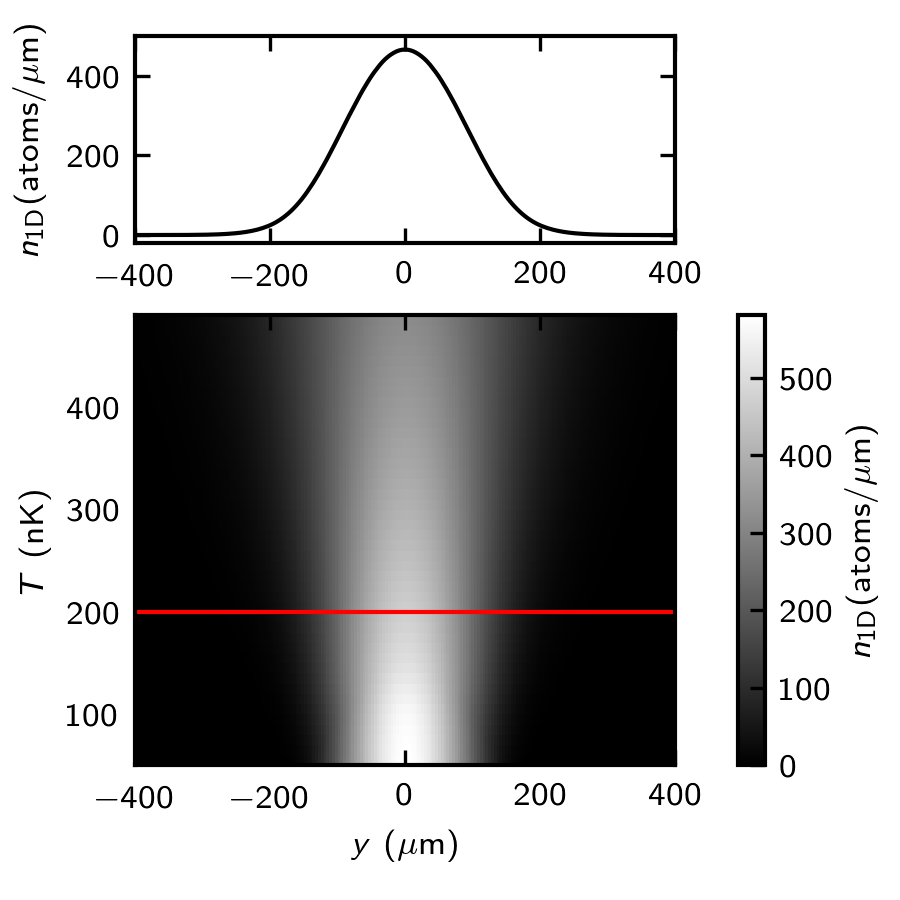
\includegraphics{{../constructClouds/N_100k_SNR_0.0_1D_density}.png}}
		{\caption{1D density profiles along longitudinal $y-$direction (see Eq.~\eqref{eq:n}) for a cloud of 100'000 atoms at various temperatures $T$. The upper part shows few exemplary curve indicated as red lines in the lower plot.}
			\label{fig:1D_density_nonoise}}
		\ffigbox[\FBwidth]{\includegraphics{../constructClouds/{N_100k_SNR_0.0_deviation}.pdf}}
		{\caption{Deviation of the second moments obtained form density profiles reconstructed from a various number of principal components (see also Eq.~~\eqref{eq:dev}).}
			\label{fig:n100ksnr0}}
	\end{floatrow}
\end{figure}
\begin{figure}
	\begin{floatrow}
		\ffigbox[\FBwidth]{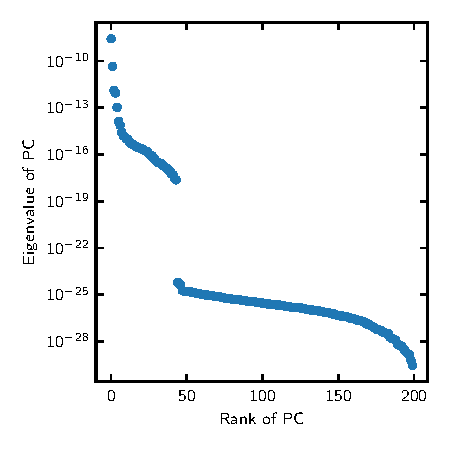
\includegraphics{{../constructClouds/N_100k_SNR_0.0_PC_eigenvalues}.pdf}}
		{\caption{Eigenvalues of the covariance matrix, sorted in descending order.}
			\label{fig:EVal_nonoise}}
		\ffigbox[\FBwidth]{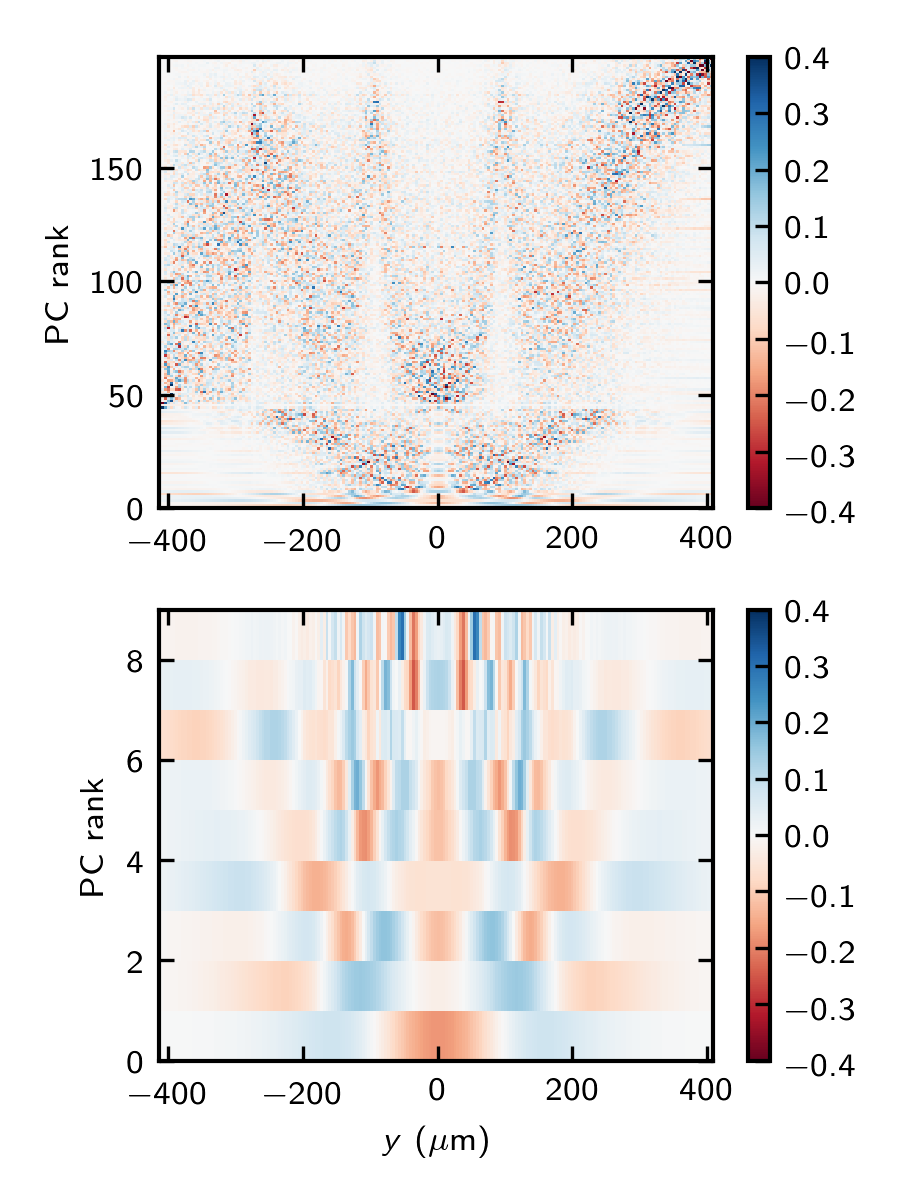
\includegraphics{{../constructClouds/N_100k_SNR_0.0_Eigenvectors}.png}}
		{\caption{Eigenvectors of the covariance matrix. The lower part shows a zoom into the first 10 EVs.}
			\label{fig:EV_nonoise}}
	\end{floatrow}
\end{figure}

Performing a PCA on the data shown in Fig.~\ref{fig:1D_density_nonoise} we find the eigenvalues shown in Fig.~\ref{fig:EVal_nonoise} and the according eigenvectors shown in Fig.~\ref{fig:EV_nonoise}. As can be seen the main structures of the profiles is given by the first few components. 

We can now reduce the dimensionality and reconstruct the density profiles from the $m$ largest principal components (see Eq.~\eqref{eq:reconstruct}). Ultimately we want to know how the value of the second moment 
\begin{equation}
	\left<y^2\right> = \int^\infty_{-\infty}\text{d}y\ n(y) y^2
\end{equation}
changes when using an increasing number of PCs. When all principal components are included in the reconstruction, the picture should be the original, and so should be the value of the second moment (can be used as a consistency check). We define the second moment obtained form density profile reconstruction $\bm{n^m} = \bm{\tilde{n}^m} + \bm{\bar{n}}$ using the $m$ larges PCs as $\left< y_m^2 \right>$ (here we have suppressed the index $i$ for better readability). The deviation of this second moment value (in percent) from the original value is plotted in Fig.~\ref{fig:n100ksnr0}:
\begin{equation}
	\mathrm{plotted\ deviation}\ (\%) = \left(\frac{\left< y_m^2 \right>}{\left< y^2 \right>} - 1\right)\cdot100
	\label{eq:dev}
\end{equation}
The fast convergence confirms that only few PCs are required to fully describe the data and specifically the second moment.


\paragraph{Constant temperature}
We repeat the analysis while fixing the temperature to \( T=\SI{100}{\nano\kelvin} \) and varying the particle number. The density profiles are shown in Fig.~\ref{fig:1D_density_nonoise_constT}. The results of the analysis are shown in Fig.~\ref{fig:n100ksnr0_constT}, \ref{fig:EVal_nonoise_constT} and \ref{fig:EV_nonoise_constT}.

%\begin{figure}
%	\fcapside{\caption{1D density profiles along longitudinal $y-$direction (see Eq.~\eqref{eq:n}) for a cloud of temperature $T=\SI{100}{\nano\kelvin}$ and atom numbers varying from \( 10^4-2\cdot10^5 \) atoms. The upper part shows an exemplary curve for $T=\SI{200}{nK}$. The upper part shows few exemplary curve indicated as red lines in the lower plot.}
%		\label{fig:1D_density_nonoise_constT}}
%	{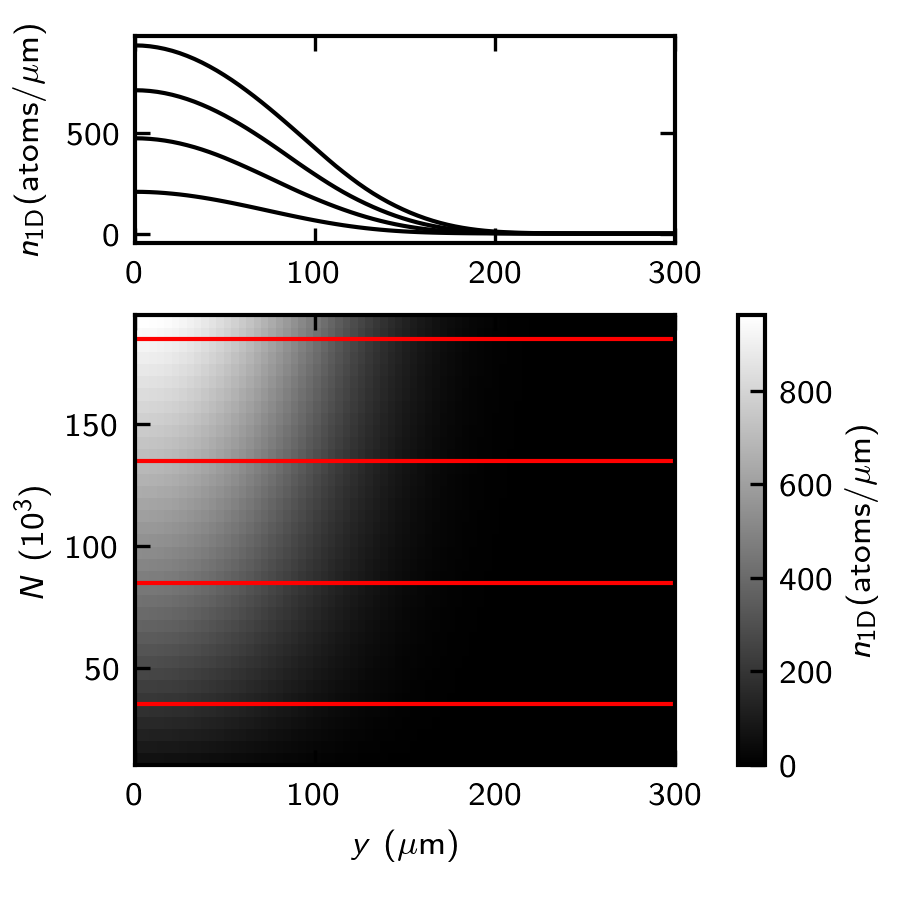
\includegraphics{{../constructClouds/T_100k_SNR_0.0_1D_density}.png}}
%\end{figure}

\begin{figure}
	\begin{floatrow}
		\ffigbox[\FBwidth]{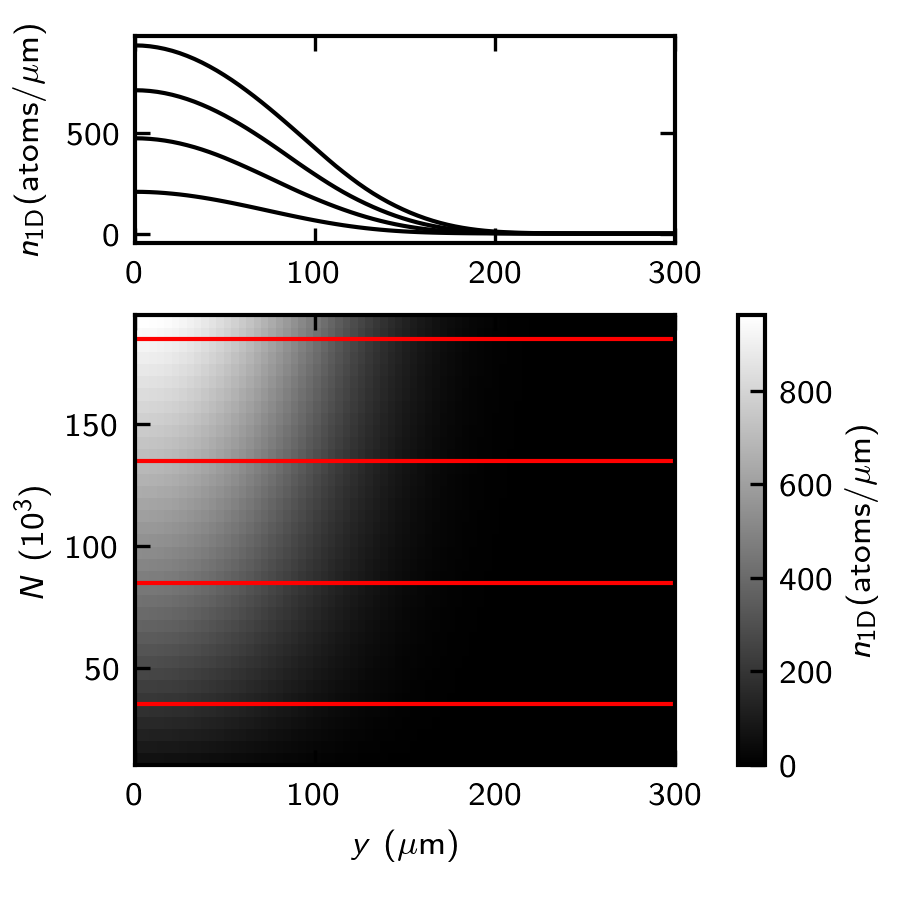
\includegraphics{{../constructClouds/T_100k_SNR_0.0_1D_density}.png}}
		{\caption{1D density profiles along longitudinal $y-$direction (see Eq.~\eqref{eq:n}) for a cloud of temperature $T=\SI{100}{\nano\kelvin}$ and atom numbers varying from \( 10^4-2\cdot10^5 \) atoms. The upper part shows an exemplary curve for $T=\SI{200}{nK}$. The upper part shows few exemplary curve indicated as red lines in the lower plot.}
			\label{fig:1D_density_nonoise_constT}}
		\ffigbox[\FBwidth]{\includegraphics{../constructClouds/{N_100k_SNR_0.0_deviation}.pdf}}
		{\caption{Deviation of the second moments obtained form density profiles reconstructed from a various number of principal components (see also Eq.~~\eqref{eq:dev}) at fixed temperature $T=\SI{100}{nK}$.}
			\label{fig:n100ksnr0_constT}}
	\end{floatrow}
\end{figure}
\begin{figure}
	\begin{floatrow}
		\ffigbox[\FBwidth]{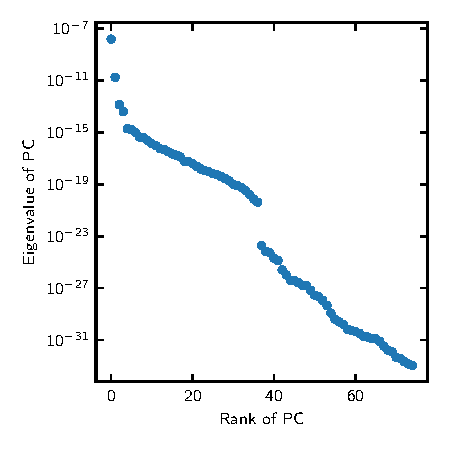
\includegraphics{{../constructClouds/T_100k_SNR_0.0_PC_eigenvalues}.pdf}}
		{\caption{Eigenvalues of the covariance matrix, sorted in descending order.}
			\label{fig:EVal_nonoise_constT}}
		\ffigbox[\FBwidth]{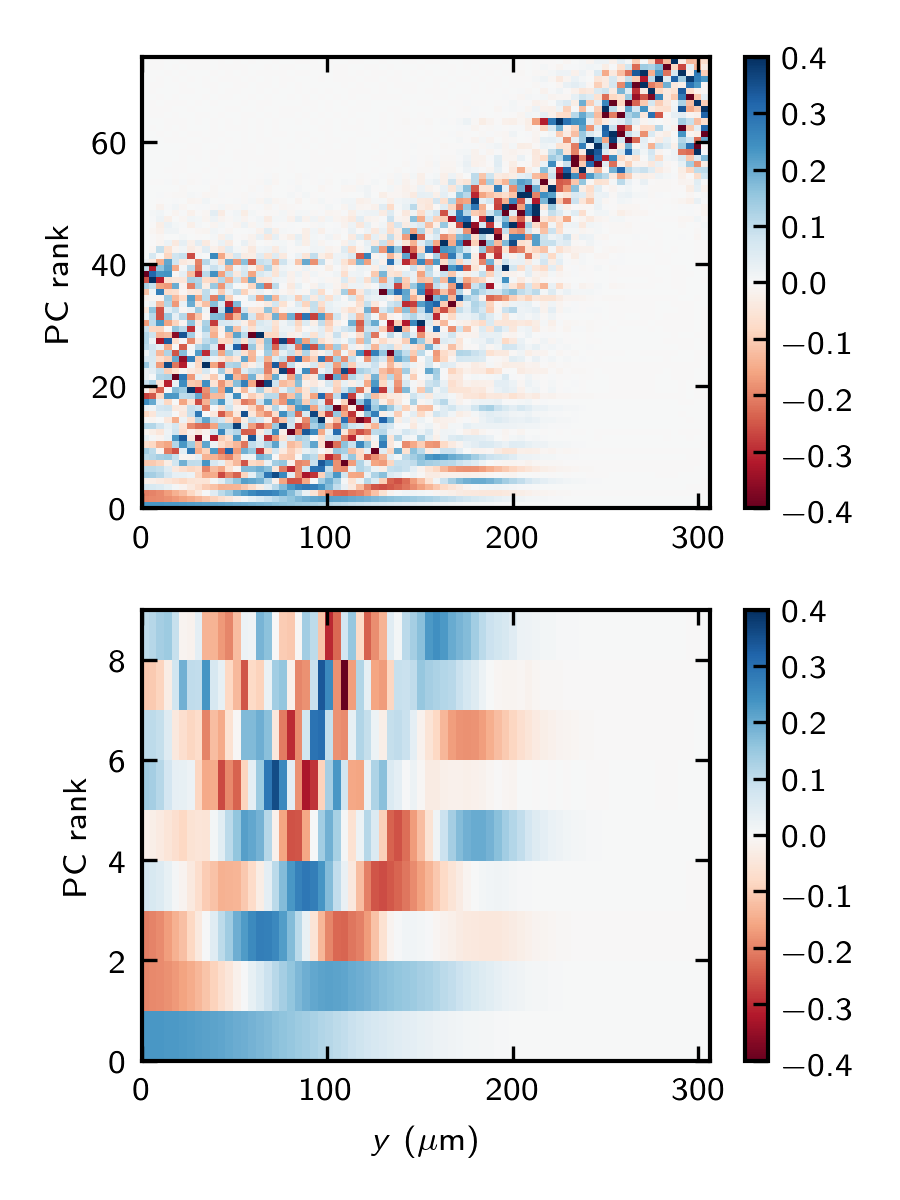
\includegraphics{{../constructClouds/T_100k_SNR_0.0_Eigenvectors}.png}}
		{\caption{Eigenvectors of the covariance matrix. The lower part shows a zoom into the first 10 EVs.}
			\label{fig:EV_nonoise_constT}}
	\end{floatrow}
\end{figure}


\newpage
\paragraph{Density profiles with noisy data}
Now we want to get to a situation closer to what is encountered in the experiment, namely we add random noise to our density pictures. Here the noise amplitude $s_0$ is quantified as fraction of the maximal signal from the density profile (the central peak). We accordingly modify the density profiles by adding this noise:
\begin{equation}
	\bm{n} \rightarrow \bm{n} + \bm{\delta n}
\end{equation}
where $\bm{\delta n}= s_0 \bm{s}$ and $\bm{s}$ is a vector of random numbers between -0.5 and 0.5, and $s_0$ indicates the magnitude of the error.

A simple repetition of PC analysis gives sobering results. 


\vfill
\newpage
\printbibliography

\end{document}